\chapter{Методы исследования \todo{...}}\label{ch:ch2}

\section{Атомно-силовая микроскопия}\label{sec:ch2/sect1}
Атомно-силовая микроскопия (АСМ) позволяет осуществлять картирование рельефа поверхности образца, а также отклика различной природы с высоким пространственным разрешением. Сканирование осуществляется с помощью иглы с радиусом закругления \(\sim\)\SI{10}{\nm}, расположенной на конце кантилевера (рис. \cref{fig:afm_cantilever}). Отклонение кантилевера при взаимодействии иглы с образцом вызывает смещение лазерного луча, отражающегося от поверхности кантилевера, которое, в свою очередь, детектируется при помощи четырёхсекционного фотоприёмника (рис. \cref{fig:afm_system}).

\begin{figure}[ht]
    \centerfloat{
        \hfill
        \subcaptionbox[List-of-Figures entry]{\label{fig:afm_cantilever} \SI{151}{\electronvolt}}{%
            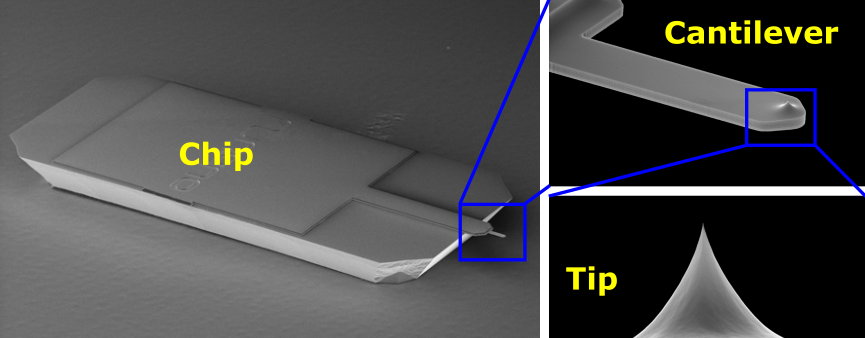
\includegraphics[width=0.5\linewidth]{afm/cantilever.png}}
        \hfill
        \subcaptionbox{\label{fig:afm_system}\SI{121}{\electronvolt}}{%
            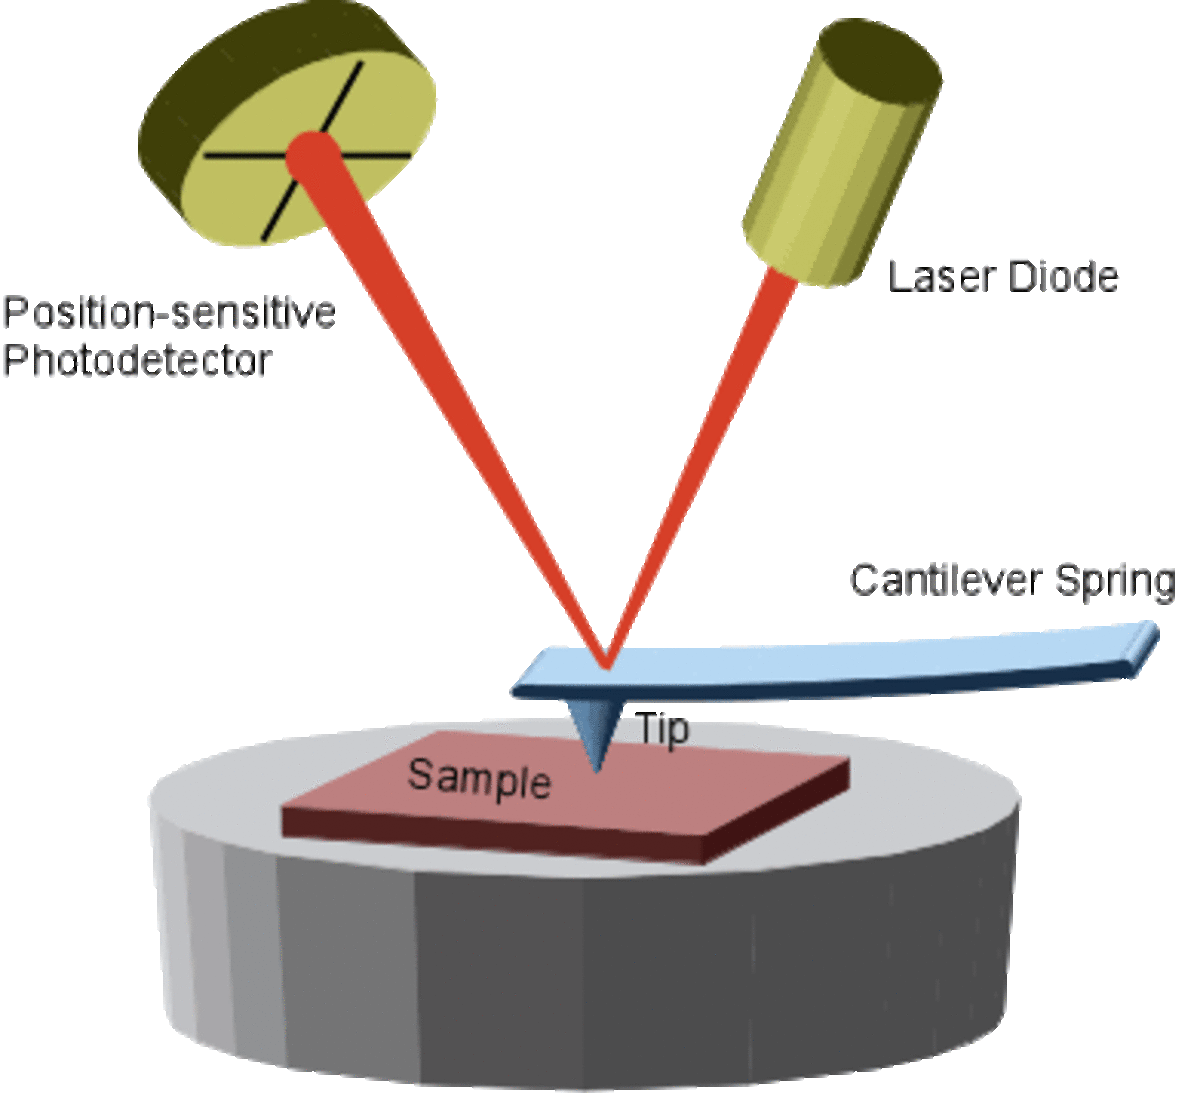
\includegraphics[width=0.5\linewidth]{afm/afm.png}}
        \hfill
    }
    \caption[Этот текст попадает в названия рисунков в списке рисунков]{Распределение атомов платины в плёнке HZO \todo{после 100 000 актов распыления} при различных энергиях распыляемых частиц}\label{fig:afm}
\end{figure}

\subsection{Микроскопия пьезоотклика}\label{sec:ch2/sect1/sub1}
Микроскопия пьезоотклика (piezoresponse force microscopy, PFM) позволяет исследовать распределение пьезоотклика в пьезоэлектрике с помощью измерения величины деформации, вызванной обратным пьезоэффектом (рис. \cref{fig:pfm}).

\begin{figure}[ht]
    \centerfloat{
        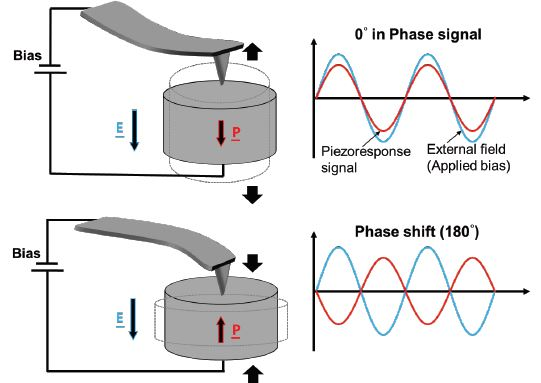
\includegraphics[width=0.6\linewidth]{pfm/pfm.jpg}
    }
    \caption{Микроскопия пьезоотклика}\label{fig:pfm}
\end{figure}

При этом возможно использование двух принципиально разных способов измерения: исследование пьезоотклика сегнетоэлектрического слоя при приложении напряжения между иглой и нижним электродом (\textit{ex citu}\todo{, рис X.Xа, нужно самому нарисовать, в solidworks например, если будешь успевать до защиты}) и исследование пьезоотклика в готовой ячейке памяти (\textit{in situ}, \todo{рис X.Xб}) при приложении напряжения между верхним и нижним электродами. При этом в случае \textit{ex citu} измерений сканируется непосредственно сегнетоэлектрическая плёнка, а в случае \textit{in situ} измерений сканируется поверхность электрода, деформирующаяся вслед за сегнетоэлектрическим слоем. Каждый из подходов имеет свои недостатки и преимущества. Так, в случае \textit{ex situ} измерений возможно \todo{протекание электрохимических реакций на поверхности сегнетоэлектрика [ref], неравномерное электрическое поле, которое к тому же в значительной степени зависит от формы иглы в момент измерения, возможно контролируемое зарождение домена с обратной поляризацией в месте контакта с зондом}, однако \textit{in situ} измерения неизбежно ухудшают пространственное разрешение ...,

\todo{Из-за слабого отклика появляется необходимость в использовании резонансных методик, а поскольку контактная резонансная частота изменяется при сканировании поверхности, возникает необходимость отслеживания резонансной частоты при измерениях, DART, BE PFM сравнение}

\todo{Для получения амплитуды и фазы отклика используется Фурье преобразование сигнала с фотоприёмника, после чего полученный спектр фильтруется и с помощью алгоритма vector fitting аппроксимируется для получения амплитуды и фазы отклика на резонасной частоте, по-хорошему сюда бы ещё картинку сырые данные -> fft -> filtered fft -> vector fit, мб у Калинина}

\subsubsection{Измерение латерального пьезоотклика}
При использовании АСМ возможно детектирование не только вертикального отклонения кантилевера, но и его изгиба относительно своей оси. Это имеет особый интерес в случае PFM измерений, поскольку позволяет получить латеральный пьезоотклик структуры \todo{рисунок}. При этом при получении карты вертикального отклика, а также карт латерального отклика в \todo{обычном} положении и при повороте образца на \ang{90}, возможно восстановить распределение трёхмерного вектора отклика, а значит и полного вектора поляризации. \todo{объяснить, зачем поворот нужен}

\subsubsection{Спектроскопия}
(Switching spectroscopy, SS PFM)

\subsubsection{Количественные измерения}
Для получения количественных результатов при PFM измерениях необходимо провести калибровку \todo{прибора, кантилевер}. Для этого используется \todo{возбуждение кантилевера в воздухе} ... термопик

\section{Электрофизические измерения}
Зондовая станция, PUND, CV, PQ (написать какие импульсы подаются, рисуночек, особенно для PQ, объяснить токи)

